\paragraph{QuizziPedia::Front-End::Controllers::UserDetailsController}
\begin{figure} [ht]
	\centering
	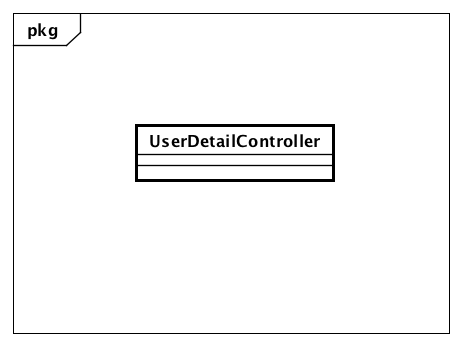
\includegraphics[scale=0.6]{UML/Classi/Front-End/QuizziPedia_Front-end_Controller_UserDetailController.png}
	\caption{QuizziPedia::Front-End::Controllers::UserDetailController}
\end{figure} \FloatBarrier
\begin{itemize}
	\item \textbf{Descrizione}: questa classe permette di gestire i dati di un utente da mostrare nella pagina di un profilo;
	\item \textbf{Utilizzo}: fornisce le funzionalità per ottenere i dati di un utente per poterle mostrare nella \textit{view\ped{G}};
	\item \textbf{Relazione con altre classi}:
	\begin{itemize}
		\item \textbf{IN \texttt{UserDetailsModelView}}: \textit{directive\ped{G}} che permette di visualizzare i dati di un utente; 
		\item \textbf{IN \texttt{UserDetailsService}}: questa classe permette di ottenere i dati dell'utente;
		\item \textbf{IN \texttt{UserDetailsModel}}: rappresenta un utente. Contiene tutte le informazioni necessarie alla presentazione del contenuto di un utente sia nella visualizzazione che nella gestione di un profilo.
	\end{itemize}
	\item \textbf{Attributi}:
	\begin{itemize}
		\item \texttt{-} \texttt{\$scope: \$scope} \\
		Campo dati contenente un riferimento all'oggetto \$scope creato da \textit{Angular\ped{G}}, viene utilizzato come mezzo di comunicazione tra il \textit{controller\ped{G}} e la \textit{view\ped{G}}. Contiene gli oggetti che definiscono il \textit{model\ped{G}} dell'applicazione;
		\item \texttt{-} \texttt{\$rootScope: \$rootScope} \\
		Campo dati contenente il riferimento all'oggetto globale \$rootScope creato da \textit{Angular\ped{G}}. Viene utilizzato per rendere accessibile a tutti i \textit{controller\ped{G}} e a tutte le \textit{view\ped{G}} l'oggetto \texttt{UserDetailsModel}. In questo caso viene utilizzato per inserire in \$rootScope l'oggetto di ritorno della chiamata a \texttt{getUserDetails} del \textit{service\ped{G}} \texttt{UserDetailsService};
		\item \texttt{-} \texttt{userDetailsService: userDetailsService} \\ Questa classe permette di ottenere i dati personali degli utenti;
		\item \texttt{+} \texttt{details: UserDetailsModelView} \\
		Oggetto di tipo \texttt{UserDetailsModelView}. All'interno di esso sono presenti le variabili e i metodi necessari per il \textit{Two-Way Data-Binding\ped{G}} tra la \textit{directive\ped{G}} \texttt{UserDetailsDirective} e il \textit{controller\ped{G}} \texttt{UserDetailsController}.
	\end{itemize}	
		\item \textbf{Metodi}:
		\begin{itemize}
		\item \texttt{+} \texttt{UserDetailsController(\$scope: \$scope, \$rootScope:\$rootScope, \$mdDialog: \$mdDialog, UserDetailsService: UserDetailsService)} \\ Metodo costruttore della classe.\\
		\textbf{Parametri}: 
		\begin{itemize}
			\item \texttt{\$scope: \$scope} \\
			Parametro contenente un riferimento all'oggetto \$scope creato da \textit{Angular\ped{G}}. Viene utilizzato come mezzo di comunicazione tra il \textit{controller\ped{G}} e la \textit{view\ped{G}}. Contiene gli oggetti che definiscono il \textit{viewmodel\ped{G}} e il \textit{model\ped{G}} dell'applicazione;
			\item \texttt{\$rootScope: \$rootScope} \\
			Parametro contenente il riferimento all'oggetto globale \$rootScope creato da \textit{Angular\ped{G}}. Viene utilizzato per rendere accessibile a tutti i \textit{controller\ped{G}} e a tutte le \textit{view\ped{G}} l'oggetto \texttt{UserDetailsModel}. In questo caso viene utilizzato per inserire in \$rootScope l'oggetto di ritorno della chiamata a \texttt{getUserDetails} del \textit{service\ped{G}} \texttt{UserDetailsService};
			\item \texttt{\$mdDialog: \$mdDialog} \\
			Campo dati contenente un riferimento al servizio della libreria \textit{Material for Angular\ped{G}} che permette di creare delle componenti a pop-up;
			\item \texttt{userDetailsService: userDetailsService}: parametro che permette di ottenere, tramite il \textit{service\ped{G}}, la lista di tutti i dati dell'utente.
		\end{itemize}
		\item \texttt{-} \texttt{getUserDetails(username: String): UserDetailsModel} \\ Metodo che permette di ottenere i dati con una chiamata a \texttt{UserDetailsService}.
		\textbf{Parametri}:
		\begin{itemize}
			\item \texttt{username: String}: parametro che identifica l'utente del quale saranno scaricati i dati.
		\end{itemize}
	\end{itemize}
\end{itemize}

